% \documentclass{article}
% \usepackage{tikz}
% \usepackage{amsmath}
% \usepackage{listings}
% \usepackage{xcolor}

\usetikzlibrary{trees, arrows.meta, positioning}
\lstset{
  basicstyle=\ttfamily\small,
  frame=single,
  backgroundcolor=\color{gray!10},
  breaklines=true,
  keywordstyle=\color{blue},
  commentstyle=\color{gray},
  stringstyle=\color{purple},
  showstringspaces=false
}

\subsection{Exercise 2 Sheet Solution (Spring 2025)}
\subsubsection{Q1. Identify the type of each tree}

\textbf{Left Tree:}
\begin{itemize}
  \item Binary Tree: \textbf{Yes}
  \item Binary Search Tree: \textbf{No} (4 is left of 2, 6 is left of 5)
  \item Balanced Tree: \textbf{No}
\end{itemize}

\textbf{Middle Tree:}
\begin{itemize}
  \item Binary Tree: \textbf{Yes}
  \item Binary Search Tree: \textbf{Yes}
  \item Balanced Tree: \textbf{No}
\end{itemize}

\textbf{Right Tree:}
\begin{itemize}
  \item Binary Tree: \textbf{Yes}
  \item Binary Search Tree: \textbf{Yes}
  \item Balanced Tree: \textbf{Yes}
\end{itemize}

\subsubsection{Q2. Construct a Binary Search Tree (BST)}

Insert values: $15, 20, 25, 18, 16, 14, 26, 27, 13, 23$

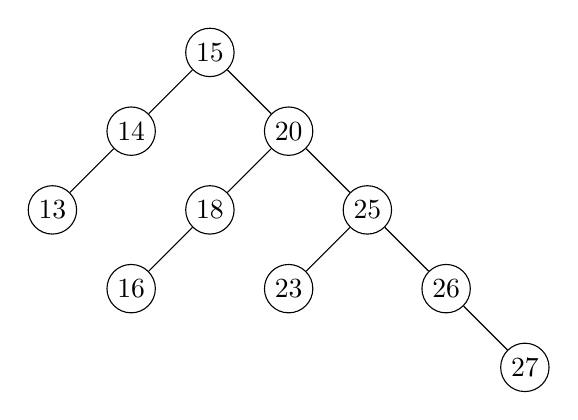
\begin{tikzpicture}[sibling distance=2cm, level distance=1cm, every node/.style={draw, circle, minimum size=6mm, inner sep=2pt}]
\node {15}
  child {node {14}
    child {node {13}}
    child[missing]
  }
  child {node {20}
    child {node {18}
      child {node {16}}
      child[missing]
    }
    child {node {25}
      child {node {23}}
      child {node {26}
        child[missing]
        child {node {27}}
      }
    }
  };
\end{tikzpicture}

\subsubsection{Q3. Delete operations on BST}

\textbf{Delete 30:} \\
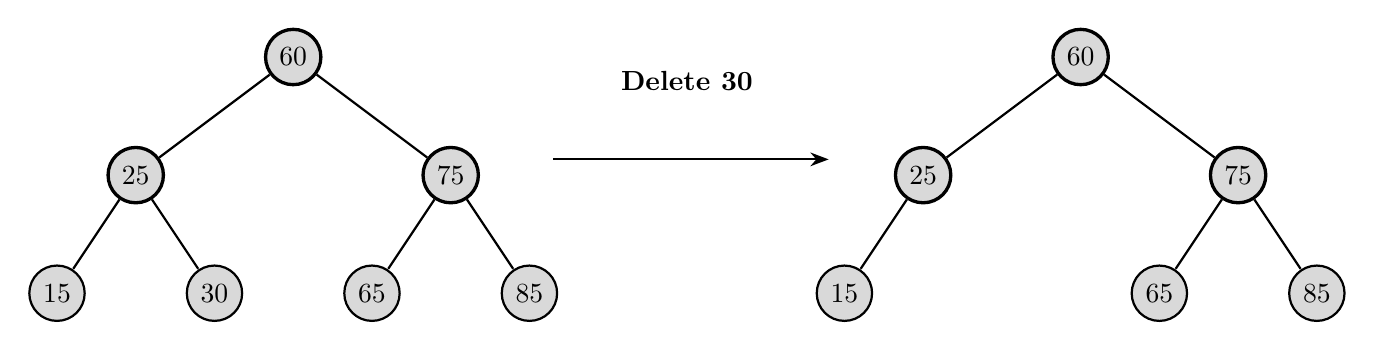
\begin{tikzpicture}[
  very thick,
  % level distance=1.3cm,
  % sibling distance=2.2cm,
  level/.style={sibling distance=40mm/#1},
  edge from parent/.style={draw, thick},
  arrow/.style={thick, ->, >=Stealth}
]
\tikzstyle{vertex}=[draw,fill=black!15,circle,minimum size=20pt,inner sep=0pt]
% Original tree
\node [vertex] at (0,0) {60}
  child {node [vertex] {25}
    child {node [vertex] {15}}
    child {node [vertex] {30}}
  }
  child {node [vertex] {75}
    child {node [vertex] {65}}
    child {node [vertex] {85}}
  };

% Arrow with label
\node (arrowtext) at (5, -0.3) {\textbf{Delete 30}};
\draw[arrow] (3.3, -1.3) -- (6.8, -1.3);

% Resulting tree
\node [vertex] at (10,0) {60}
  child {node [vertex] {25}
    child {node [vertex] {15}}
    child [missing]
  }
  child {node [vertex] {75}
    child {node [vertex] {65}}
    child {node [vertex] {85}}
  };

\end{tikzpicture}

\textbf{Delete 25:}
\[
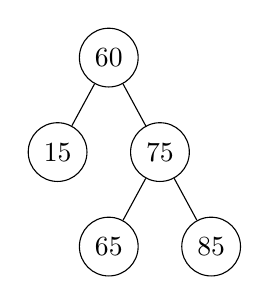
\begin{tikzpicture}[level distance=1.2cm, sibling distance=1.3cm, every node/.style={draw, circle}]
\node {60}
  child {node {15}}
  child {node {75}
    child {node {65}}
    child {node {85}}
  };
\end{tikzpicture}
\]

\textbf{Delete 60 (Way 1):}
\[
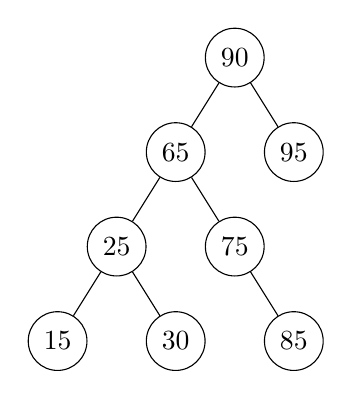
\begin{tikzpicture}[level distance=1.2cm, sibling distance=1.5cm, every node/.style={draw, circle}]
\node {90}
  child {node {65}
    child {node {25}
      child {node {15}}
      child {node {30}}
    }
    child {node {75}
      child[missing]
      child {node {85}}
    }
  }
  child {node {95}};
\end{tikzpicture}
\]

\textbf{Delete 60 (Way 2):}
\[
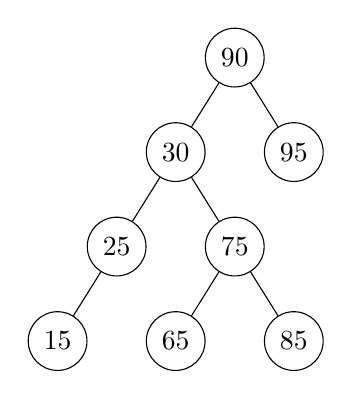
\begin{tikzpicture}[level distance=1.2cm, sibling distance=1.5cm, every node/.style={draw, circle}]
\node {90}
  child {node {30}
    child {node {25}
      child {node {15}}
      child[missing]
    }
    child {node {75}
      child {node {65}}
      child {node {85}}
    }
  }
  child {node {95}};
\end{tikzpicture}
\]

\subsubsection{Q4. Traversals}

Tree:
\[
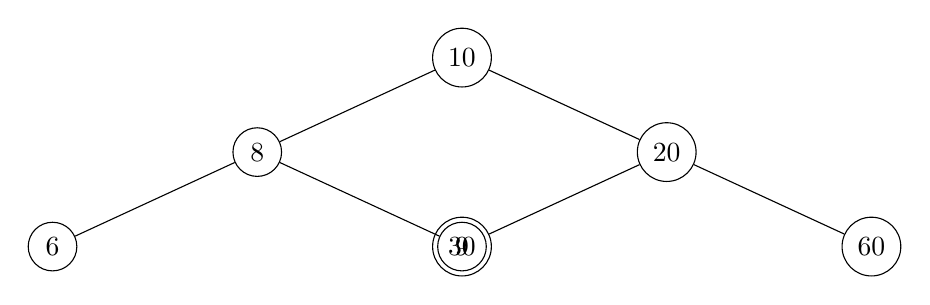
\begin{tikzpicture}[level distance=1.2cm, sibling distance=5.2cm, every node/.style={draw, circle}]
\node {10}
  child {node {8}
    child {node {6}}
    child {node {9}}
  }
  child {node {20}
    child {node {30}}
    child {node {60}}
  };
\end{tikzpicture}
\]

\textbf{Answers:}
\begin{itemize}
  \item In-order: $6\ 8\ 9\ 10\ 20\ 30\ 60$
  \item Pre-order: $10\ 8\ 6\ 9\ 20\ 30\ 60$
  \item Post-order: $6\ 9\ 8\ 20\ 30\ 60\ 10$
\end{itemize}

\subsubsection{Q5. Binary Tree Node Count and Height}

\begin{itemize}
  \item (a) Max nodes in perfect tree of height 10: $2^{10} - 1 = 1023$
  \item (b) Height of tree with $10^6$ nodes: $\log_2(10^6 + 1) \approx 20$
\end{itemize}

\subsubsection{Q6. Tree Formula Representation}

Tree shown in figure:
\[
T = \text{Fork}(40, \text{Fork}(15, \text{Fork}(10, \text{Fork}(3, \text{EMPTY}, \text{EMPTY}), \text{EMPTY}),\\ 
\text{Fork}(30, \text{EMPTY}, \text{Fork}(36, \text{EMPTY}, \text{EMPTY}))),\\
\text{Fork}(50, \text{Fork}(51, \text{EMPTY}, \text{EMPTY}), \text{EMPTY}))
\]

\subsubsection{Q7. Tree from Pseudocode Insert}

\textbf{Given:} \_array = [25, 36, 6, 6, 18, 10, 15, 35]

\textbf{1. Traversals:}
\begin{itemize}
  \item In-order: $6, 10, 15, 18, 25, 35, 36$
  \item Pre-order: $25, 6, 18, 10, 15, 36, 35$
\end{itemize}

\textbf{2. Height after inserting 19:} 5

\textbf{3. Max nodes without increasing height:} $2^5 - 1 = 31$

\textbf{4. Can we construct a balanced tree of same length?} Yes.

Example array: $[10,10,5,3,6,15,11,16]$

Tree:
\[
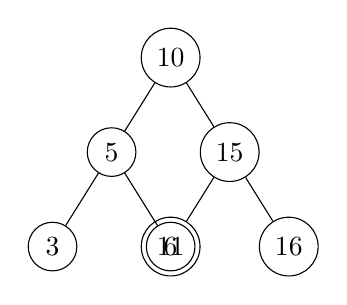
\begin{tikzpicture}[level distance=1.2cm, sibling distance=1.5cm, every node/.style={draw, circle}]
\node {10}
  child {node {5}
    child {node {3}}
    child {node {6}}
  }
  child {node {15}
    child {node {11}}
    child {node {16}}
  };
\end{tikzpicture}
\]

\subsubsection{Q8. Tree Visit Procedure Analysis}
Consider a procedure that visits the elements of a tree and constructs a list with these elements. Let us define a function \texttt{visit}:

\begin{quote}
\begin{tt}
visit($\Box$) = [ ] \\
visit(Fork($x, l, r$)) = visit($r$) + [$x$] + visit($l$)
\end{tt}
\end{quote}

where $[\ldots]$ denotes a list of elements. In particular, the special case $[\,]$ denotes the empty list and operation $+$ denotes concatenation of lists. For example, $[3, 4, 1] + [2, 3, 5]$ results in $[3, 4, 1, 2, 3, 5]$.

Consider a function named \texttt{doSomething} that takes an array of integers $a$ with $n$ elements (that is, \texttt{a.length = n}) and first inserts these elements in a binary search tree and then constructs a list using the function \texttt{visit}.

\begin{lstlisting}
List doSomething(int [] a) {
    Tree T = null;
    for (int i = 0; i < a.length; i++) {
        assert (#nodes(T) == i); // invariant
        T = insert(T, A[i]);
    }
    List L = visit(T);
    assert (length(L) == a.length); // postcondition
    return L;
}
\end{lstlisting}

(Note that function \texttt{\#nodes(T)} returns the number of nodes in tree T and function \texttt{length(L)} returns the number of elements in list L.)

---

\subsection*{(a) Briefly describe the task this algorithm performs.}

\textbf{Answer:}  
The algorithm inserts all elements from the input array into a binary search tree and then generates a list of these elements in \textbf{descending order}, effectively sorting the input elements and removing duplicates.

---

\subsection*{(b) The invariant and the postcondition do not always hold true. Under what condition would they fail?}

\textbf{Answer:}  
If the input array contains duplicate values (e.g., $[1, 2, 2, 3, 4]$), the invariant would fail on the 3rd iteration, when the duplicate '2' is not inserted again, so \#nodes(T) remains 2 instead of increasing to 3.

Likewise, the postcondition \texttt{length(L) == a.length} will also fail, since L will only contain the unique inserted elements, not all from the input array.

Therefore, both the invariant and postcondition hold \textbf{only if the input array has no duplicates} or if the \texttt{insert()} function allows duplicates.

---

\subsection*{(c) What is the worst-case time complexity of \texttt{doSomething}?}

\textbf{Answer:}  
In the worst case, if the binary search tree is unbalanced (like a linked list), inserting each element will take $O(n)$ time. Since we do this for $n$ elements, the total time is:

\[
O(n \cdot n) = O(n^2)
\]

Thus, the worst-case time complexity of \texttt{doSomething} is $O(n^2)$.



\textbf{(a)} The algorithm inserts all elements from the input array into a BST and then outputs the elements in \textbf{descending order}, removing duplicates.

\textbf{(b)} The invariant/postcondition fail if duplicates exist in the array — the tree will skip inserting them, reducing the node count while still incrementing the loop counter.

\textbf{(c)} Worst-case time complexity is $O(n^2)$:
- Outer loop: $O(n)$
- Insert into unbalanced BST: worst case $O(n)$ per insert
- Overall: $n \times n = O(n^2)$


% \begin{tikzpicture}[very thick,level/.style={sibling distance=60mm/#1}]
% \tikzstyle{vertex}=[draw,fill=black!15,circle,minimum size=20pt,inner sep=0pt]
% \node [vertex] (r){$17$}
%   child {
%     node [vertex] (a) {$19$}
%     child {
%       node [vertex] {$20$}
%       child {
%         node [vertex] {$-3$}
%         child {node [vertex] {$17$}}
%         child {node [vertex] {$5$}}
%       }
%       child {node [vertex] {$6$}}
%     }
%     child {
%       node [vertex] {$3$}
%       child {node [vertex] {$7$}}
%       child {node [vertex] {$2$}}
%     }
%   }
%   child {
%     node [vertex] {$9$}
%     child {
%       node [vertex] {$8$}
%       child [missing]
%       child {node [vertex] {$2$}}
%     }
%     child {
%       node [vertex] {$11$}
%       child {node [vertex] {$17$}}
%       child {node [vertex] {$-4$}}
%     }
%   };
% \end{tikzpicture}


